% From: https://texample.net/tikz/examples/complete-graph/

% A complete graph
% Author: Quintin Jean-Noël
% <http://moais.imag.fr/membres/jean-noel.quintin/>
\documentclass{article}
\usepackage{tikz}
\usetikzlibrary[topaths]
% A counter, since TikZ is not clever enough (yet) to handle
% arbitrary angle systems.
\newcount\mycount
\begin{document}
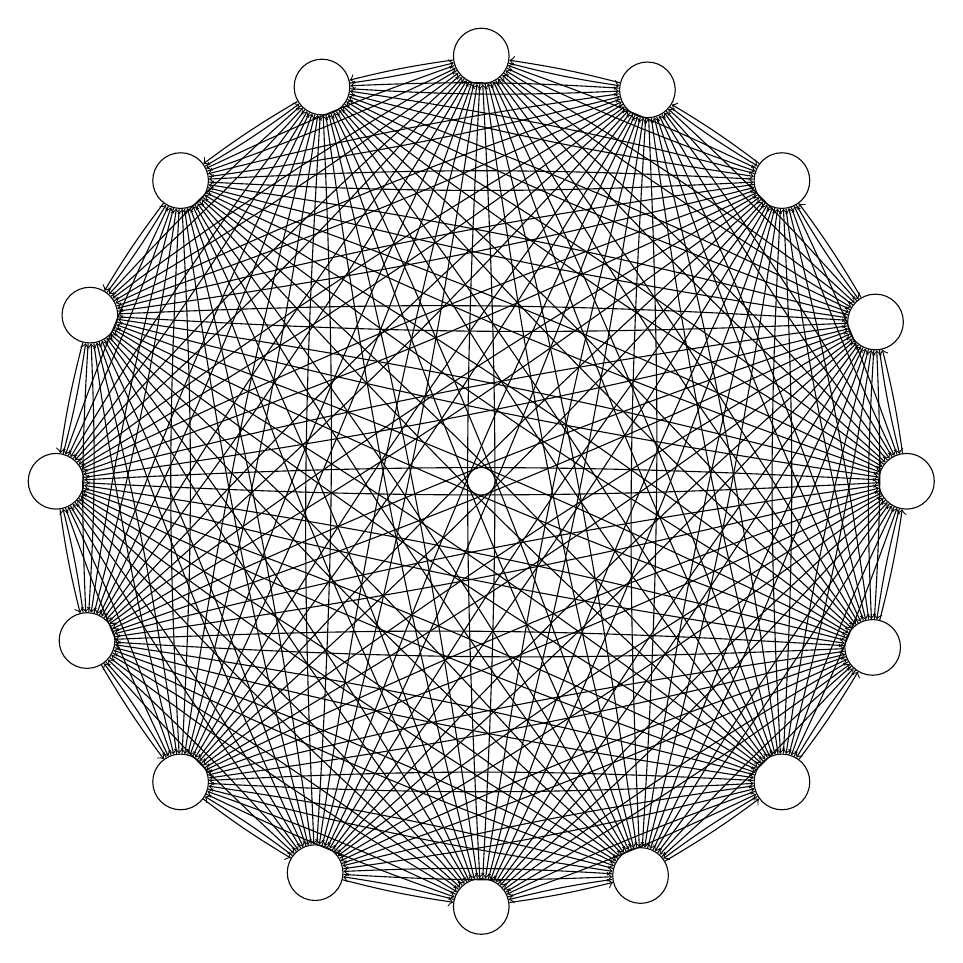
\begin{tikzpicture}[transform shape]
  %the multiplication with floats is not possible. Thus I split the loop in two.
  \foreach \number in {1,...,8}{
      % Computer angle:
        \mycount=\number
        \advance\mycount by -1
  \multiply\mycount by 45
        \advance\mycount by 0
      \node[draw,circle,inner sep=0.25cm] (N-\number) at (\the\mycount:5.4cm) {};
    }
  \foreach \number in {9,...,16}{
      % Computer angle:
        \mycount=\number
        \advance\mycount by -1
  \multiply\mycount by 45
        \advance\mycount by 22.5
      \node[draw,circle,inner sep=0.25cm] (N-\number) at (\the\mycount:5.4cm) {};
    }
  \foreach \number in {1,...,15}{
        \mycount=\number
        \advance\mycount by 1
  \foreach \numbera in {\the\mycount,...,16}{
    \path (N-\number) edge[->,bend right=3] (N-\numbera)  edge[<-,bend
      left=3] (N-\numbera);
  }
}
\end{tikzpicture}
\end{document}
